\chapter{Thesis}
\label{cha:Diplomschrift}

\section{The Vehicle}

The DeepRacer itself represents a core part of this thesis, as it is used to test the trained models in a real-world environment. Our school acquired two of these cars. one of which we are using for this thesis. Below is a list of all parts included with one DeepRacer vehicle.

\begin{enumerate}
    \item Vehicle chassis
    \item Vehicle body cover
    \item Compute module battery
    \item Power cable and power adapter
    \item Vehicle battery
\end{enumerate}

\subsection{Chassis and Accessories}
The vehicle itself consists primarily of a four wheel drive chassis which holds all other components. The chassis can be further separated into a lower part, which contains the brushed electric motor, and an upper part that carries the compute module and a power bank to supply it \cite{AWS19}. The entire car is build on a scale of 1/18 to a real car, meaning proportions like distance between wheels were kept realistic. This is especially apparent while driving, as one would expect better manoeuvrability and smaller turning radius.

At the front there are three USB ports used to mount the camera and other equipment like keyboards. As a crucial part of any self-driving car, the camera provided with the DeepRacer provides a 4-megapixel image directly to the compute module. Since we are working with the first edition of the DeepRacer vehicle and not with the newer DeepRacer Evo, which has stereo cameras and a LiDAR\footnote{Light detection and ranging} sensor, object avoidance and head-to-head racing are not supported by default. It is however possible to purchase an upgrade kit for 249,00 US\$, which includes an additional stereo camera and the LiDAR sensor.

The front wheel steering is controlled by a servomechanism \cite{AWS19}. Correctly configuring the steering proved to be a very difficult task, as we were unable to align both front wheels so that the car would drive in a straight line. The configuration is done via a web interface hosted by the compute module. Using this interface, the maximum steering angles can be configured to fit the physical vehicle. Our problem however doesn't stem from the configuration interface, but rather from the vehicle itself. The front wheels are not aligned properly, which leads to one wheel being either to far left or right. This causes the car to have a left-hand twist or right-hand twist, respectively. As of writing this, we haven't been able to solve this issue.

\subsection{Compute Module}
The upper component houses the ``brain'' of our car. The compute module consists of an Intel Atom
%todo: Fix trademark symbol
processor, 4 Gigabyte of RAM and 32 Gigabyte of memory, which can be expanded upon via a SD card. This hardware is running Linux Ubuntu 16.04.3 with Intel OpenVINO\textsc{TM} and ROS\footnote{Robot Operating System} Kinetic. Apart from that the chassis offers 4 USB type A ports, 1 USB type C port, 1 Micro-USB port and one HDMI port. The USB type C port is used to supply the compute module with power, while the HDMI port offers the ability to connect a display and directly access the modules operating system.

In addition to that, the compote module hosts its own web interface, from which the vehicle can be monitored, remotely controlled and configured.
% maybe insert image of DeepRacer console here

\section{The physical Track}

Being able to drive along a simulation of the track is only a partial success. In order to prove successful, the trained algorithm is required to complete multiple runs on a real track using our DeepRacer vehicle. We decided on rebuilding the track used 2018 during the AWS re:Invent.

The circular track starts with a 180° left turn, followed by a right-starting s-curve and continues on with two left turns back to the beginning. With a total width of 7.93 m and length of 5.18 m it impractical to paint it on a single, solid piece.

Before we considered building the track, we painted it on the floor in our robotics laboratory. This was possible due to the floor being solid black, just like the road on the track.

Rather than that we chose to use interlocking foam pieces which are lightweight and easy to store and transport.

\begin{figure}
    \centering
    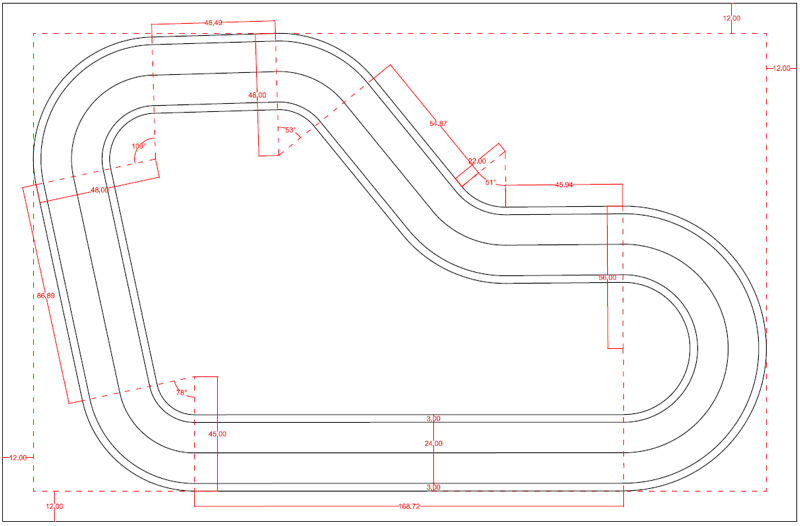
\includegraphics[width=.85\textwidth]{deepracer-track-2018-guideline.png}
    \caption{AWS re:Invent 2018 track}
    \label{fig:track}
\end{figure}

\section{Machine Learning and Autonomous Driving}


 \section{Local Training}
 
 One of the major drawbacks of using the DeepRacer in a learning environment are the costs of training. Amazon offers easy, albeit functionally limited ways of training RL models in their cloud services. This sort of contradicts the intended use, as the DeepRacer is supposed to offer a simple and affordable entry into the ways of machine learning. Below is the pricing table. \footnote{Cited date 2020/08/20}
 \begin{table}
 \caption{Pricing for model training with AWS services.}
 \label{tab:services}
 \centering
 \setlength{\tabcolsep}{5mm}
 \def\arraystretch{1.25}
 \begin{tabular}{|r|r|c|c|c|}
 \hline
 \textbf{service} & \textbf{pricing} \\
 \hline\hline
 training and evaluation & 3.50 US\$ per hour \\
 \hline
 model storage & 0.023 US\$ per GB \\
 \hline
 \end{tabular}
 \end{table}
 In order to circumvent this cost barrier we -- like others before us -- began setting up a training environment on one of the more powerful computers in the robotics lab.
 The setup for local training is available on GitHub \footcite{https://github.com/aws-deepracer-community/deepracer}. In order to function properly the computer had to meet the following requirements:
 \begin{itemize}
 \item A Linux distribution, preferably Ubuntu
 \item NVIDIA grafic processor and proper dirvers
 \item Docker
 \item Python
 \item Minio, a S3 simulator
 \end{itemize}